\documentclass[main.tex]{subfiles}

\begin{document}

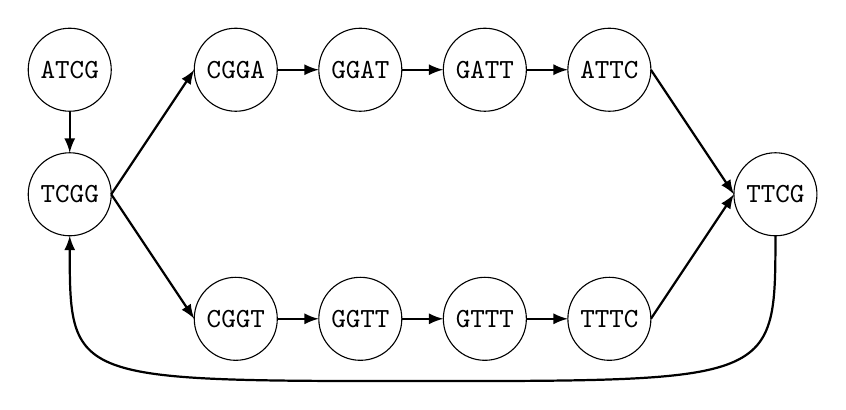
\begin{tikzpicture}[x=0.75pt,y=0.75pt,yscale=-1,xscale=1]

% begin part
\draw (0, 0) circle (20) node {\texttt{ATCG}};
\draw [fill opacity=1, ->, >=latex,thick,black] (0, 20) -- (0, 40);
\draw (0, 60) circle (20) node {\texttt{TCGG}};

\draw [fill opacity=1, ->, >=latex,thick,black] (20, 60) -- (60, 0);
\draw [fill opacity=1, ->, >=latex,thick,black] (20, 60) -- (60, 120);

% second part
\draw (80, 0) circle (20) node {\texttt{CGGA}};
\draw [fill opacity=1, ->, >=latex,thick,black] (100, 0) -- (120, 0);
\draw (140, 0) circle (20) node {\texttt{GGAT}};
\draw [fill opacity=1, ->, >=latex,thick,black] (160, 0) -- (180, 0);
\draw (200, 0) circle (20) node {\texttt{GATT}};
\draw [fill opacity=1, ->, >=latex,thick,black] (220, 0) -- (240, 0);
\draw (260, 0) circle (20) node {\texttt{ATTC}};

% third part
\draw (80, 120) circle (20) node {\texttt{CGGT}};
\draw [fill opacity=1, ->, >=latex,thick,black] (100, 120) -- (120, 120);
\draw (140, 120) circle (20) node {\texttt{GGTT}};
\draw [fill opacity=1, ->, >=latex,thick,black] (160, 120) -- (180, 120);
\draw (200, 120) circle (20) node {\texttt{GTTT}};
\draw [fill opacity=1, ->, >=latex,thick,black] (220, 120) -- (240, 120);
\draw (260, 120) circle (20) node {\texttt{TTTC}};

% merge part
\draw [fill opacity=1, ->, >=latex,thick,black] (280, 0) -- (320, 60);
\draw [fill opacity=1, ->, >=latex,thick,black] (280, 120) -- (320, 60);
\draw (340, 60) circle (20) node {\texttt{TTCG}};

\draw [->, >=latex,thick,black] (340, 80) .. controls (340, 150) and (340, 150) .. (170, 150) .. controls (0, 150) and (0, 150) .. (0, 80);

\end{tikzpicture}

\end{document}

